\documentclass[14pt]{extarticle}
\usepackage[
left=25mm,
top=20mm,
right=15mm,
bottom=20mm,
]{geometry}

\usepackage[pdftex]{graphicx}
\usepackage[utf8x]{inputenc}
\usepackage[russian]{babel}
\usepackage[T1]{fontenc}
\usepackage{float}
\usepackage{cite}
\usepackage{hyperref}
\usepackage{etoolbox}
\usepackage{indentfirst}
\usepackage{algpseudocode}
\usepackage{algorithm}
\usepackage{setspace}
\usepackage{listings}
\sloppy

\lstset{
sensitive=true,
basicstyle=\small,
keywordstyle=\color{black},
commentstyle=\scriptsize\rmfamily,
keywordstyle=\ttfamily\underbar,
identifierstyle=\ttfamily,
basewidth={0.5em,0.5em},
columns=fixed,
fontadjust=true,
literate={->}{{$\to$}}1
}

\makeatletter
%\renewcommand{\@biblabel}[1]{#1.} % Заменяем библиографию с квадратных скобок на точку:
\makeatother
\gappto\captionsrussian{\renewcommand{\contentsname}{Оглавление}}
\renewcommand\baselinestretch{1.5}
\renewcommand{\lstlistingname}{Листинг}

\begin{document}

\begin{titlepage}
\thispagestyle{empty}
\def\baselinestretch{1.0}
\begin{center}
  {САНКТ-ПЕТЕРБУРГСКИЙ ГОСУДАРСТВЕННЫЙ УНИВЕРСИТЕТ \\ \vskip 0.3em {\large Математико-механический факультет \\ \vskip 0.7em{\large Кафедра системного программирования \\}}}
    \vspace*{0.15\textheight}
    {\large Бакрадзе Лиана Георгиевна}
    
    \vskip 2em
    {\huge Дисциплина инициирования сборок мусора}
    
    \vskip 1em
    {\large Курсовая работа} \\
    \vskip 2em
    {\normalsize \raggedleft 
    Научный руководитель:\\
    к.ф.-м.н. Д.Ю. Булычев
    \\[3em]
    %Рецензент:\\
    %Неизвестно \\
    \vspace*{0.08\textheight}
    {\centering Санкт-Петербург \\ 2014}
    }
\end{center}
\end{titlepage}

\tableofcontents
\thispagestyle{empty} 
\pagebreak
\section*{Введение}

В последнее время языки, поддерживающие автоматическое управление памятью, т.е. сборку 
мусора, становятся всё более популярны. В связи с этим очень актуален вопрос о влиянии
поведения сборщика мусора на производительность приложений.

Во время реализации сборщика мусора приходится принимать много решений,
связанных с его работой: выбор алгоритма выделения памяти, устройство кучи, 
алгоритм сборки мусора, критерий вызова сборщика мусора, будет ли сборщик мусора 
перемещать объекты. Эти решения очень сильно влияют как на работу сборщика мусора, 
так и на
производительность приложений, которые его используют.

Одним из существенно влияющих на работу сборщика мусора параметров
является частота его вызовов. Если 
сборщик мусора будет вызываться слишком часто, то это может привести к неоправданно
большим накладным расходам: приложение будет постоянно приостанавливаться, но при 
этом памяти будет освобождаться во время каждого вызова мало. Если, наоборот, вызывать 
сборщик мусора слишком редко, то сборка мусора может занимать длительное время. 

Частота вызовов
зависит от дисциплины инициации сборки мусора. Можно, например, инициировать сборку
мусора только в случае, если не хватает памяти для создания новых объектов, но это может 
оказаться слишком редким для приложения, а можно вызывать через определённые интервалы времени.
Нельзя придумать универсальной стратегии, которая подходила бы для всех приложений, поэтому
необходимо
предоставлять возможности для ручной настройки параметров работы сборщика мусора. 

В рамках проекта Лаборатории языковых инструментов компании JetBrains на математико-механическом 
факультете
Санкт-Петербургского государственного университета был реализован собственный сборщик
мусора для
инфраструктуры постороения компиляторов LLVM~\cite{llvm-text}. Для того, чтобы им можно
было пользоваться,
необходимо было среди прочего разработать критерий, когда и при каких условиях он будет 
вызываться, и предоставить возможности для ручной настройки параметров.

Целью данной работы явилось изучение различных подходов к инициированию сборки мусора,
а также реализация нескольких из них в сборщике мусора для LLVM, предоставление 
возможности переключения между ними и задания их параметров.

\pagebreak
\section {Обзор существующих критериев}

Технология сборки мусора была впервые применена в среде программирования для языка
Lisp\footnote{http://en.wikipedia.org/wiki/Lisp\_(programming\_language)} и описана 
в статье~\cite{Lisp}. Сборка мусора иниицировалась в этой среде, как только не находилось
свободного блока для выделения памяти следующему объекту. 



В статье~\cite{BDW} описывается дисциплина инициирования, реализованная в
широко используемом сборщике мусора
Boehm-Demers-Weiser\footnote{http://www.hboehm.info/gc/}~(\textit{BDW}). 
Когда не находится свободного блока подходящего размера, для того, чтобы выделить память 
под новый объект,
в зависимости от значения специальной переменной FDS (\textit{free space divisor}) 
принимается решение,
вызывать или нет сборщик мусора. Сборщик мусора вызывается тогда, когда объём выделенной за прошеднее с предыдущего цикла сборки мусора
время памяти не меньше, чем определяемая FSD часть кучи. Это позволяет  уменьшить накладные расходы на сборку мусора и не приостанавливать
приложение в тех случаях, когда с прошлого цикла сборки мусора не успело образоваться
достаточно ``умерших'' объектов. Алгоритм \ref{BDW-algo} описывает этот подход к инициированию сборки мусора: 

\begin{algorithm}[hbt]
\caption{BDW}
\label{BDW-algo}
\begin{algorithmic}[1]
\If {failed to allocate new block}
    \If {allocated since last GC >= (heap size/FSD)}  
        \State collect garbage
    \Else 
        \State grow heap by((heap size/FSD) + requested size)
    \EndIf
\EndIf
%\EndProcedure
\end{algorithmic}
\end{algorithm}

Заметим, что значение FSD используется также и для определения того, насколько будет увеличена куча.
Встречаются модификации описанного алгоритма, в которых решение, во сколько раз увеличивается куча
при необходимости, принимается на основании значения ещё одной переменной.

Авторы статьи~\cite{BDW} также предложили собственный подход к инициированию сборки мусора.
Они предлагают определять несколько порогов, влияющих на решение о вызове сборщика мусора:
\begin{enumerate}
\item{Пока объём использованной памяти не достиг первого порога, сборка мусора не вызывается и куча
увеличивается, если не удалось выделить новый блок памяти.}
\item{Сборка мусора вызывается всегда, когда объём использованной памяти достигает каждого из
порогов в первый раз.}
\item{Если объём использованной памяти достиг порога $T_i$ не в первый раз, то сборщик мусора
вызовется в случае, если в предыдущий раз, когда вызвался сборщик мусора по причине
достижения этого порога, удалось освободить
значительное количество памяти.}

\end{enumerate}


Эксперименты показали, что реализация описанного подхода позволила улучшить производительность 
большинства приложений по сравнению с обычным BWD.


В статье~\cite{microphase} в качестве наиболее распространённого подхода упоминается 
подход, основанный на объёме занятой памяти в куче.
Согласно этому подходу, вызов сборки мусора происходит в том случае,
когда объём использованной памяти в куче достигает заданного порога. С помощью
изменения порога можно сильно влиять на частоту вызова сборщика мусора и объём потребляемой приложением
памяти.

Авторы статьи~\cite{microphase} замечают, что подход, основанный на объёме 
использованной памяти, приводит к тому, что сборщик мусора вызывается тогда, 
когда приложение только что выделило память для большого числа объектов, так что
сборка мусора приведёт к большим накладным расходам. Основываясь на гипотезе о том, 
в работе приложения можно выделить фазу выделения объектов и фазу ``умирания'' объектов,
авторы статьи предложили вызывать сборщик мусора в конце фазы ``умирания''. Утверждается,
что таким образом можно уменьшить накладные расходы на сборку мусора.
Для обнаружения фазы ``умирания''объектов был предложен следующий критерий: в этой
фазе длительное время не происходит выделения памяти для объектов или происходит маленькое 
количество выделений памяти. Этот оригинальный подход был реализован в виртуальной машине 
HotSpot\footnote{http://openjdk.java.net/groups/hotspot/}для 
языка Java, благодаря чему было показано,
что его применение позволило улучшить производительность тринадцати тестовых наборов. 


Авторы статьи~\cite{time-triggered} предложили стратегию для управления
вызовами действующего одновременно с программой в отдельном потоке
(\textit{concurrent}) сборщика мусора,
работа которого характеризуется временем начала и конца текущего цикла сборки мусора.
Предложенная стратегия основывается на подсчёте моментов времени, к которым
сборщик мусора должен завершить текущий цикл сборки. При этом в данной статье 
доказана теорема о верхней границе времени завершения текущего цикла сборки мусора,
которая гарантирует, что в системе будет достаточно доступной памяти. Зависимость этого
подхода только от времени исполнения является большим преимуществом, так как позволяет
использовать для управления вызовами сборщика мусора стандартный механизм управления
потоками. 
\pagebreak[4]
\section{Описание реализации}

При динамическом управлении памятью память под объекты отводится в специальной 
области памяти, называемой кучей. 

В качестве кучи сборщик мусора, о котором идёт речь в данной работе, использует
широко известную реализацию -- так называемый 
\textit{Doug Lea's malloc}\footnote{http://g.oswego.edu/dl/html/malloc.html}.
По результатам
многих независимых тестов это одна из лучших реализаций 
по скорости, фрагментации, локальности доступа и настраиваемости~\cite{Zorn}. 
Эта реализация представляет собой один файл исходного кода на языке С. 

Для того, чтобы пользователь мог во время запуска приложения задавать дисциплину 
инициирования
сборки мусора, внутри реализации кучи было написано несколько функций-обёрток, 
вызовами которых 
заменяется вызов пользовательской программой функции \texttt{malloc} для выделения памяти. 
В момент, когда
пользовательская программа впервые запрашивает блок памяти, исходя из объявленных
при запуске переменных окружения, определяется стратегия, которая будет использована 
для инициирования сборки мусора (каждая стратегия в реализации также представлена 
отдельной функцией-обёрткой), и параметры, соответствующие выбранной стратегии. 
Дисциплина инициирования сборки 
мусора определяется значением переменной окружения \texttt{GC\_STRATEGY}. Также при запуске 
можно определить общий для всех стратегий параметр, характеризующий то, во сколько раз
при необходимости будет увеличена куча. Этот параметр является целым числом
и определяется значением переменной окружения \texttt{IF}
(\textit{Increase Factor}). 

По умолчанию последний блок в использованной реализации кучи считается блоком бесконечно
большого размера, а для отслеживания необходимости вызова сборки мусора
необходимо было ограничить размер кучи. Для этой цели была написана собственная инициализация
функции \texttt{MORECORE}, которая не запрашивает память у операционной системы в случае, если можно
в соответствий с выбранной стратегией осуществить сборку мусора. Первоначальный размер кучи можно задать
в переменной окружения \texttt{HEAP\_SIZE} (по умолчанию равен 4096 байт).

Всего в рамках данной работы было реализовано четыре различных дисциплины
инициирования сборки мусора. В последующих разделах их работа описана подробно.

\subsection{Дисциплина \textit{``no space''}}
Как уже замечалось в обзоре, самым простым подходом к инициированию
сборки мусора является вызов сборки мусора, когда в куче не осталось 
свободных блоков. Отсутствие свободных блоков можно определить по тому,
что после очередного вызова вместо адреса выделенного блока \texttt{malloc} вернёт
\texttt{null}. В случае, если это произошло, в данной реализации вызывается сборка мусора,
после которой снова делается попытка выделить блок запрошенного размера.
Если и после сборки мусора в куче не нашлось нужного блока, размер кучи
увеличивается во столько раз, сколько записано в переменной \texttt{IF},
значение которой либо задано пользователем при запуске, либо определено
по умолчанию равным двойке.
Работу данной стратегии можно описать алгоритмом \ref{algo-no-space}:


\begin{algorithm}[hbt]
\caption{No space gc}
\label{algo-no-space}
\begin{algorithmic}[3]
\If {failed to allocate new block}
        \State trigger gc
        \If {failed to allocate new block}
            \State expand the heap in IF times
        \EndIf
\EndIf
\end{algorithmic}
\end{algorithm}

Ввиду простоты реализации и низких накладных расходов на сборку мусора
данная стратегия выбрана в качестве стратегии по умолчанию.
Если пользователь хочет запустить приложение со сборщиком мусора,
использующим данную стратегию, значение переменной окружения \textt{GC\_STRATEGY}
определять не нужно. Данной стратегии в реализации соответствует 
функция-обёртка \texttt{no\_space\_malloc}.



\subsection{Дисциплина \textit{``space based''}}
Для некоторых приложений вызов сборщика мусора на основе \textit{``no space''}-стратегии
может оказаться слишком редким. 

\textit{``Space based''}-стратегия основана на несложной модификации 
\textit{``no space''}-стратегии и позволяет с помощью специального параметра 
регулировать частоту вызовов сборщика мусора.
Модификация заключается в том, что сборщик мусора вызывается, когда
объём занятой памяти в куче достигает некоторого 
заданного порога, определяемого переменной окружения  \texttt{Threshold} (по умолчанию
равно 0.75). При \texttt{Threshold} равном единице мы получаем \textit{``no space''}-стратегию.
Если после сборки мусора в куче не нашлось нужного блока, размер кучи
увеличивается во столько раз, сколько записано в переменной \textit{IF}.
Работа данной стратегии описана алгоритмом~\ref{space based gc}.

\begin{algorithm}[hbt]
\caption{space based gc}
\label{space based gc}
\begin{algorithmic}[4]

\If {allocated space >= threshold * HEAP SIZE}
    \State trigger gc
\EndIf
\If {failed to allocate new block}
        \State trigger gc
\EndIf
\If {failed to allocate new block and there was no gc}
            \State trigger gc
\EndIf
\If {failed to allocate new block and there was gc}
    \State expand the heap in IF times
\EndIf 
\end{algorithmic}
\end{algorithm}


Данной стратегии в реализации соответствует функция-обёртка \textt{space\_based\_malloc}.
При работе приложения сборщик мусора будет использовать данную стратегию,
если переменная окружения \texttt{GC\_STRATEGY} равна \textt{SPACE\_BASED}.


\subsection{Дисциплина \textit{``time based''}}

На основе идеи, предложенной авторами статьи~\cite{microphase}, был разработан критерий
вызова сборщика мусора, основанный на времени работы программы. Его суть заключается
в том, что сборщик мусора вызывается, когда обнаруживается пауза в выделениях памяти.
Мы считаем, что пауза произошла, если интервал между вызовами соответствующей обёртки для \textt{malloc}
становится долгим. Сказанное можно представить в виде формулы:
    $$\frac {T_i - T_{i-1}} {T_{i-1} - T_{i-2}} > \delta $$ 
    где $T_{i}$ -- квант времени, ассоциированный с вызовом $i$-го malloc, $\delta$ -- некоторый 
    заранее заданный порог.

Понятно, что частота вызова данного сборщика мусора зависит от параметра $\delta$, 
которую пользователь может задать при запуске (по умолчанию 1.5).
Работу данного критерия можно описать алгоритмом \ref{time}. 

\begin{algorithm}
\caption{Time-based gc}
\label{time}
\begin{algorithmic}[3]
\If {Pause is detected}  
    \State Trigger gc
\EndIf
\State Try to allocate memory
\If {Failed}
    \State Expand the heap in IF times
\EndIf

\end{algorithmic}
\end{algorithm}

В реализации описанному критерию соответствует обёртка \textitt{timed\_malloc}. Для того, чтобы использовать
данный критерий, значение переменной окружения \texttt{GC\_STRATEGY} при запуске программы должно быть 
равным \texttt{TIME\_BASED}.

\subsection{Дисциплина \textit{``bdw''}} 

Также была реализована модификация стратегии, используемой в сборщике мусора 
Boehm-Demers-Weiser и описанной в статье~\cite{BDW}. 
Сборщик мусора вызывается тогда, когда объём выделенной за прошедшее с предыдущего
цикла сборки мусора
время памяти не меньше, чем определяемая FSD часть кучи, но в отличие от 
базового алгоритма для определения того, во сколько раз будет расширена куча 
при необходимости, используется переменная \texttt{IF}, а не \texttt{FSD}. Алгоритм \ref{BDW-algo1}
описывает этот подход к инициированию сборки мусора. 

\begin{algorithm}[hbt]
\caption{BDW}
\label{BDW-algo1}
\begin{algorithmic}[1]
\If {failed to allocate new block}
    \If {allocated since last GC >= (heap size/FSD)}  
        \State collect garbage
    \Else 
        \State expand heap in IF times
    \EndIf
\EndIf
%\EndProcedure
\end{algorithmic}
\end{algorithm}

В реализации данной стратегии соответствует функция-обёртка \texttt{bdw\_malloc}. Для использования
этой стратегии нужно определить переменную \texttt{GC\_STRATEGY} равной \texttt{BDW}. Также можно при запуске приложения
определить параметры \texttt{FSD} и \texttt{IF}.

\pagebreak
\newpage
\newpage
\section{Результаты}

Ниже представлены и описаны результаты, полученные при работе написанного на 
подмножестве языка OCaml приложениия \texttt{parser} со сборщиком мусора,
использующим реализованные в рамках данной работы дисциплины инициирования.
Приложение \texttt{parser} является
синтаксическим анализатором для ``игрушечного'' языка \texttt{L} и иллюстрирует типичное
поведение функциональной программы: на вход приложение получает программу на языке 
\texttt{L}
и строит для неё синтаксическое дерево. 


Для анализа влияния дисциплины инициирования сборки мусора на частоту вызова сборщика
мусора для каждой из стратегий был построен график, изображающий продолжительность 
вызванных сборкой мусора пауз в 
работе приложения. На рисунках \ref{pic:pause-no-gc},
\ref{pic:space-based-pause}, \ref{pic:time-based-pause}, \ref{pic:pause-bdw} 
изображены такие графики для каждой из стратегий соответственно. Высота столбца на графиках
соответствует продолжительности паузы. Из представленных графиков видно, что
стратегия \textit{``bdw''} обеспечивает наиболее редкий вызов сборщика мусора, что сказывается,
однако, на продолжительности пауз, делая их достаточно долгими. 
Большая продолжительность пауз при использовании этой стратегии вызвана
тем, что во время каждой паузы освобождается много объектов в куче,
благодаря чему эта стратегии имеет самые низкие накладные расходы на сборку
мусора. Наиболее частые паузы характерны для \textit{``space based''}-сборщика мусора. 

На рисунке \ref{pic:allocated} представлено распределение занятой памяти во время работы 
приложения, а на \ref{pic:perf} время работы приложения в зависимости
от использованной дисциплины инициирования сборок мусора. Из этого рисунка видно, что дисциплина вызова 
\textit{``time based''} обеспечивает наилучшее время работы приложения, что, возможно,
связанно с тем, что она не требует обхода кучи для определения, необходимо 
ли вызывать сборщик мусора. В случае, если к среде исполнения предъявляется требование
по экономному расходу доступной памяти, следует использовать \textit{``space based''}-сборщик
мусора, который обеспечивает самый маленький объём занятой памяти.

Исходя из полученных результатов, можно сделать следующие выводы:
\begin{itemize}
\item cамой эффективной по времени является дисциплина инициирования сборки мусора
\textit{``time based''};
\item cамой эффективной по использованию памяти является дисциплина инициирования
сборки мусора \textit{``space based''};
\item cамые маленькие накладные расходы на сборку мусора обеспечивает
дисциплина инициирования \textit{``bdw''}.
\end{itemize}

\begin{figure}[ph]
\caption{\label{pic:pause-no-gc}распределение пауз при работе no gc}
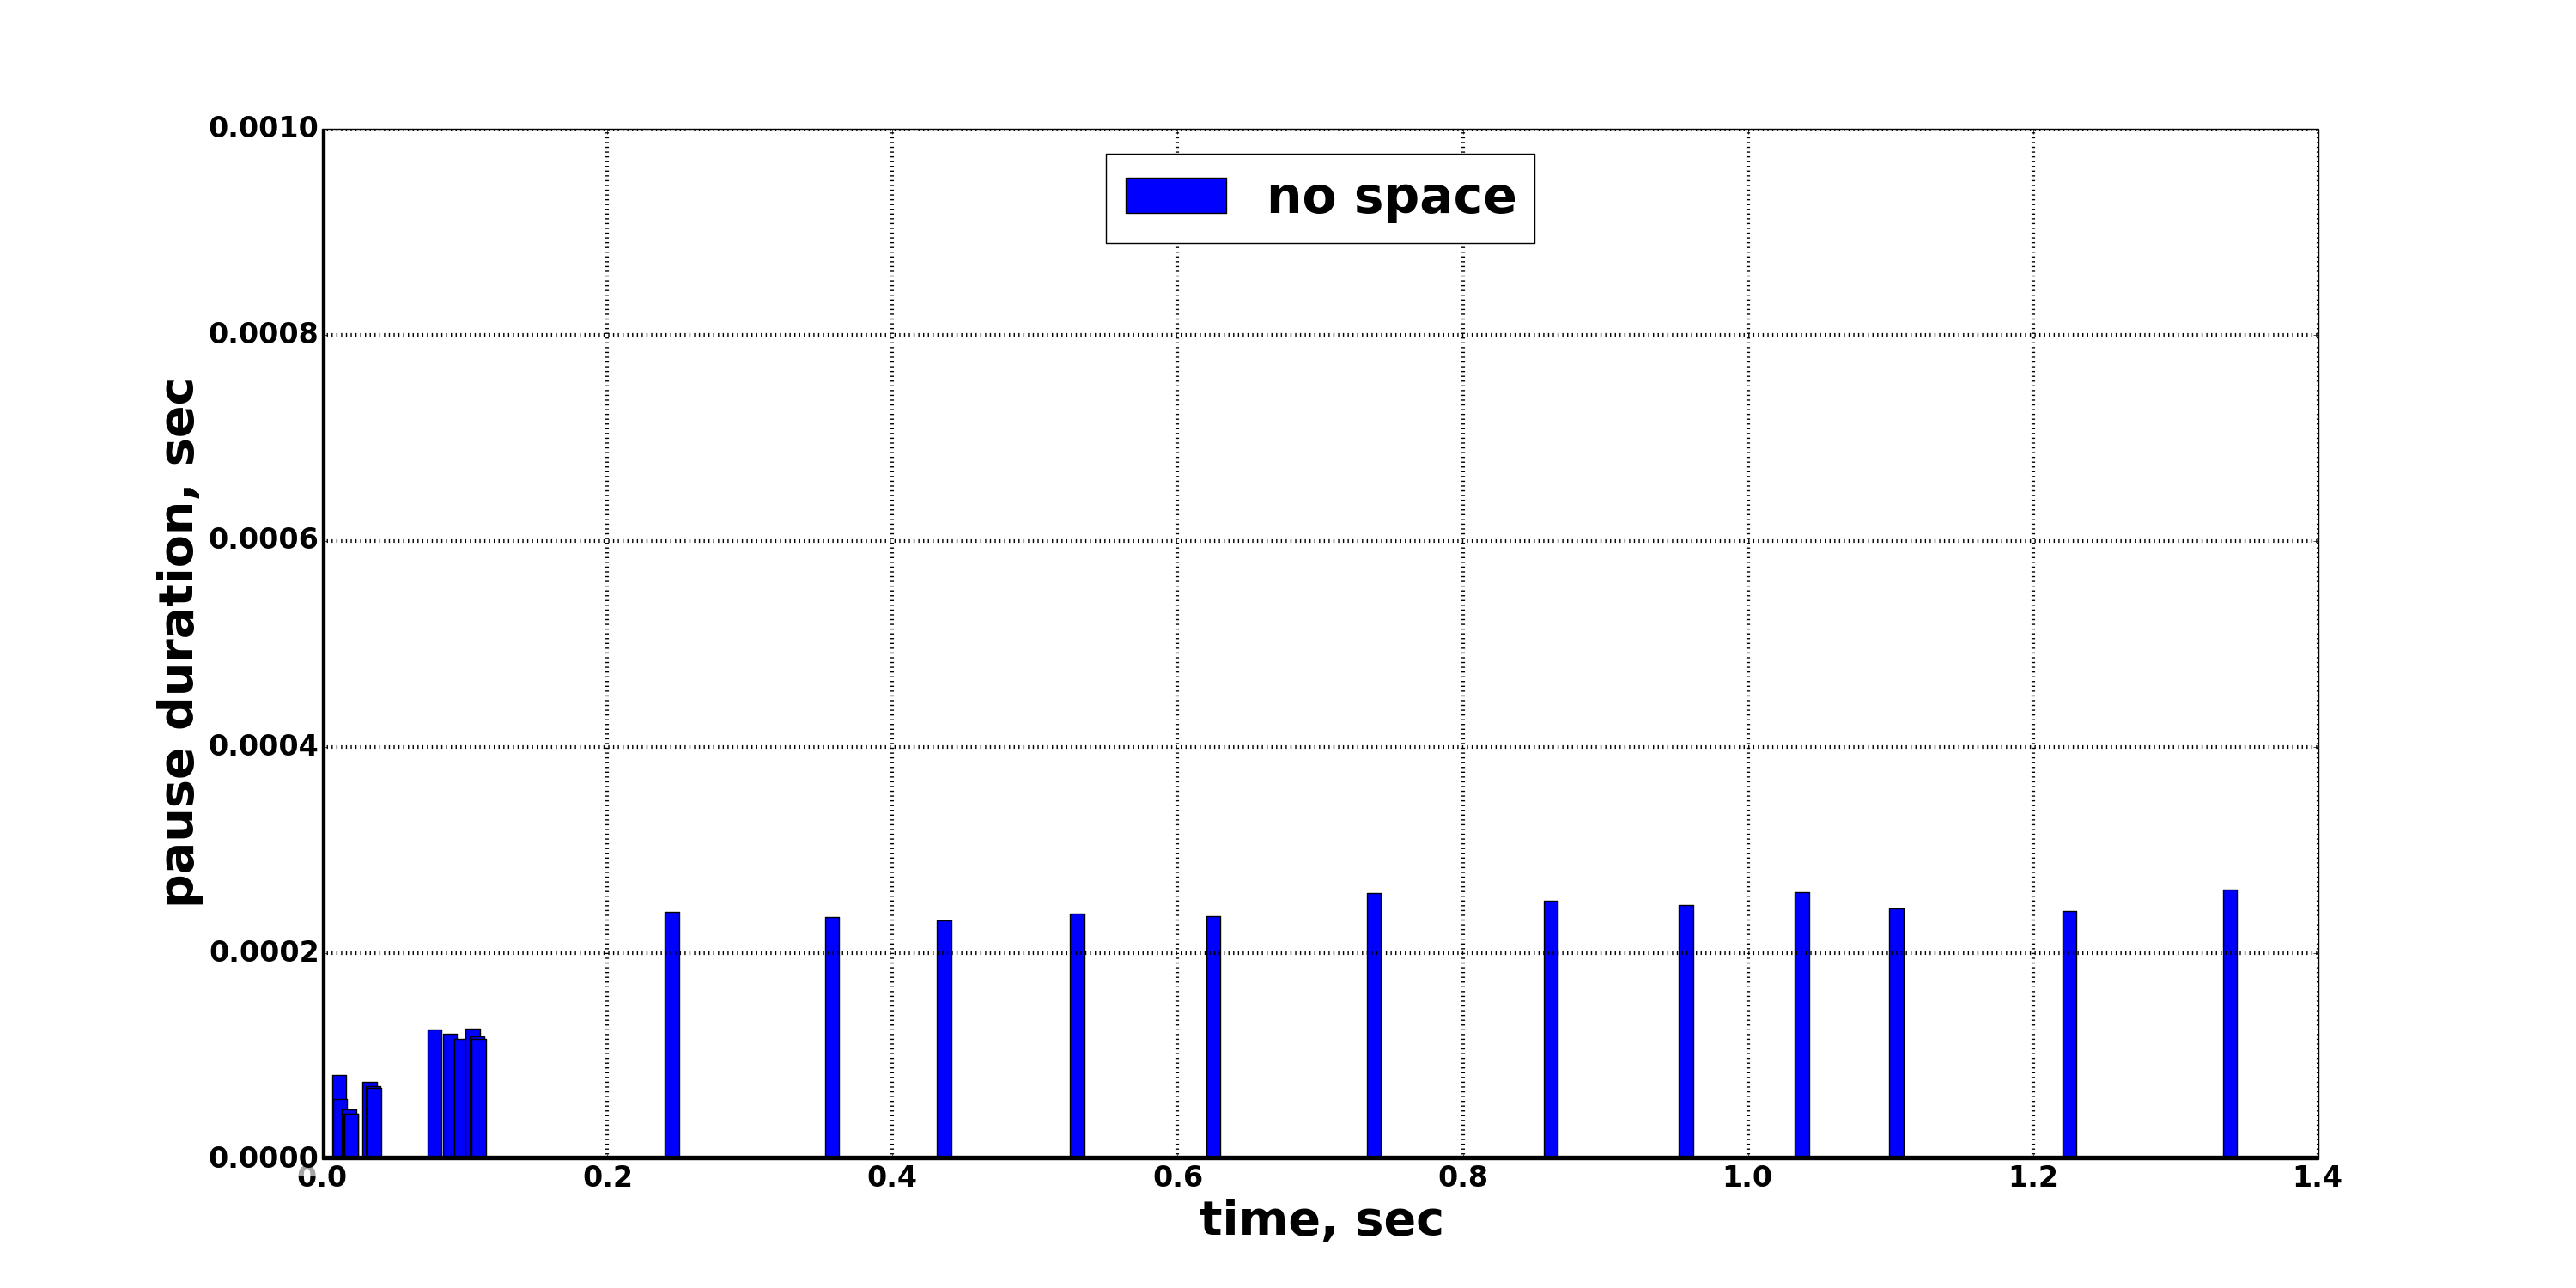
\includegraphics[width=1\linewidth]{no-apce.png}
\end{figure}

\begin{figure}[ph]
\caption{\label{pic:space-based-pause}распределение пауз при работе space based}
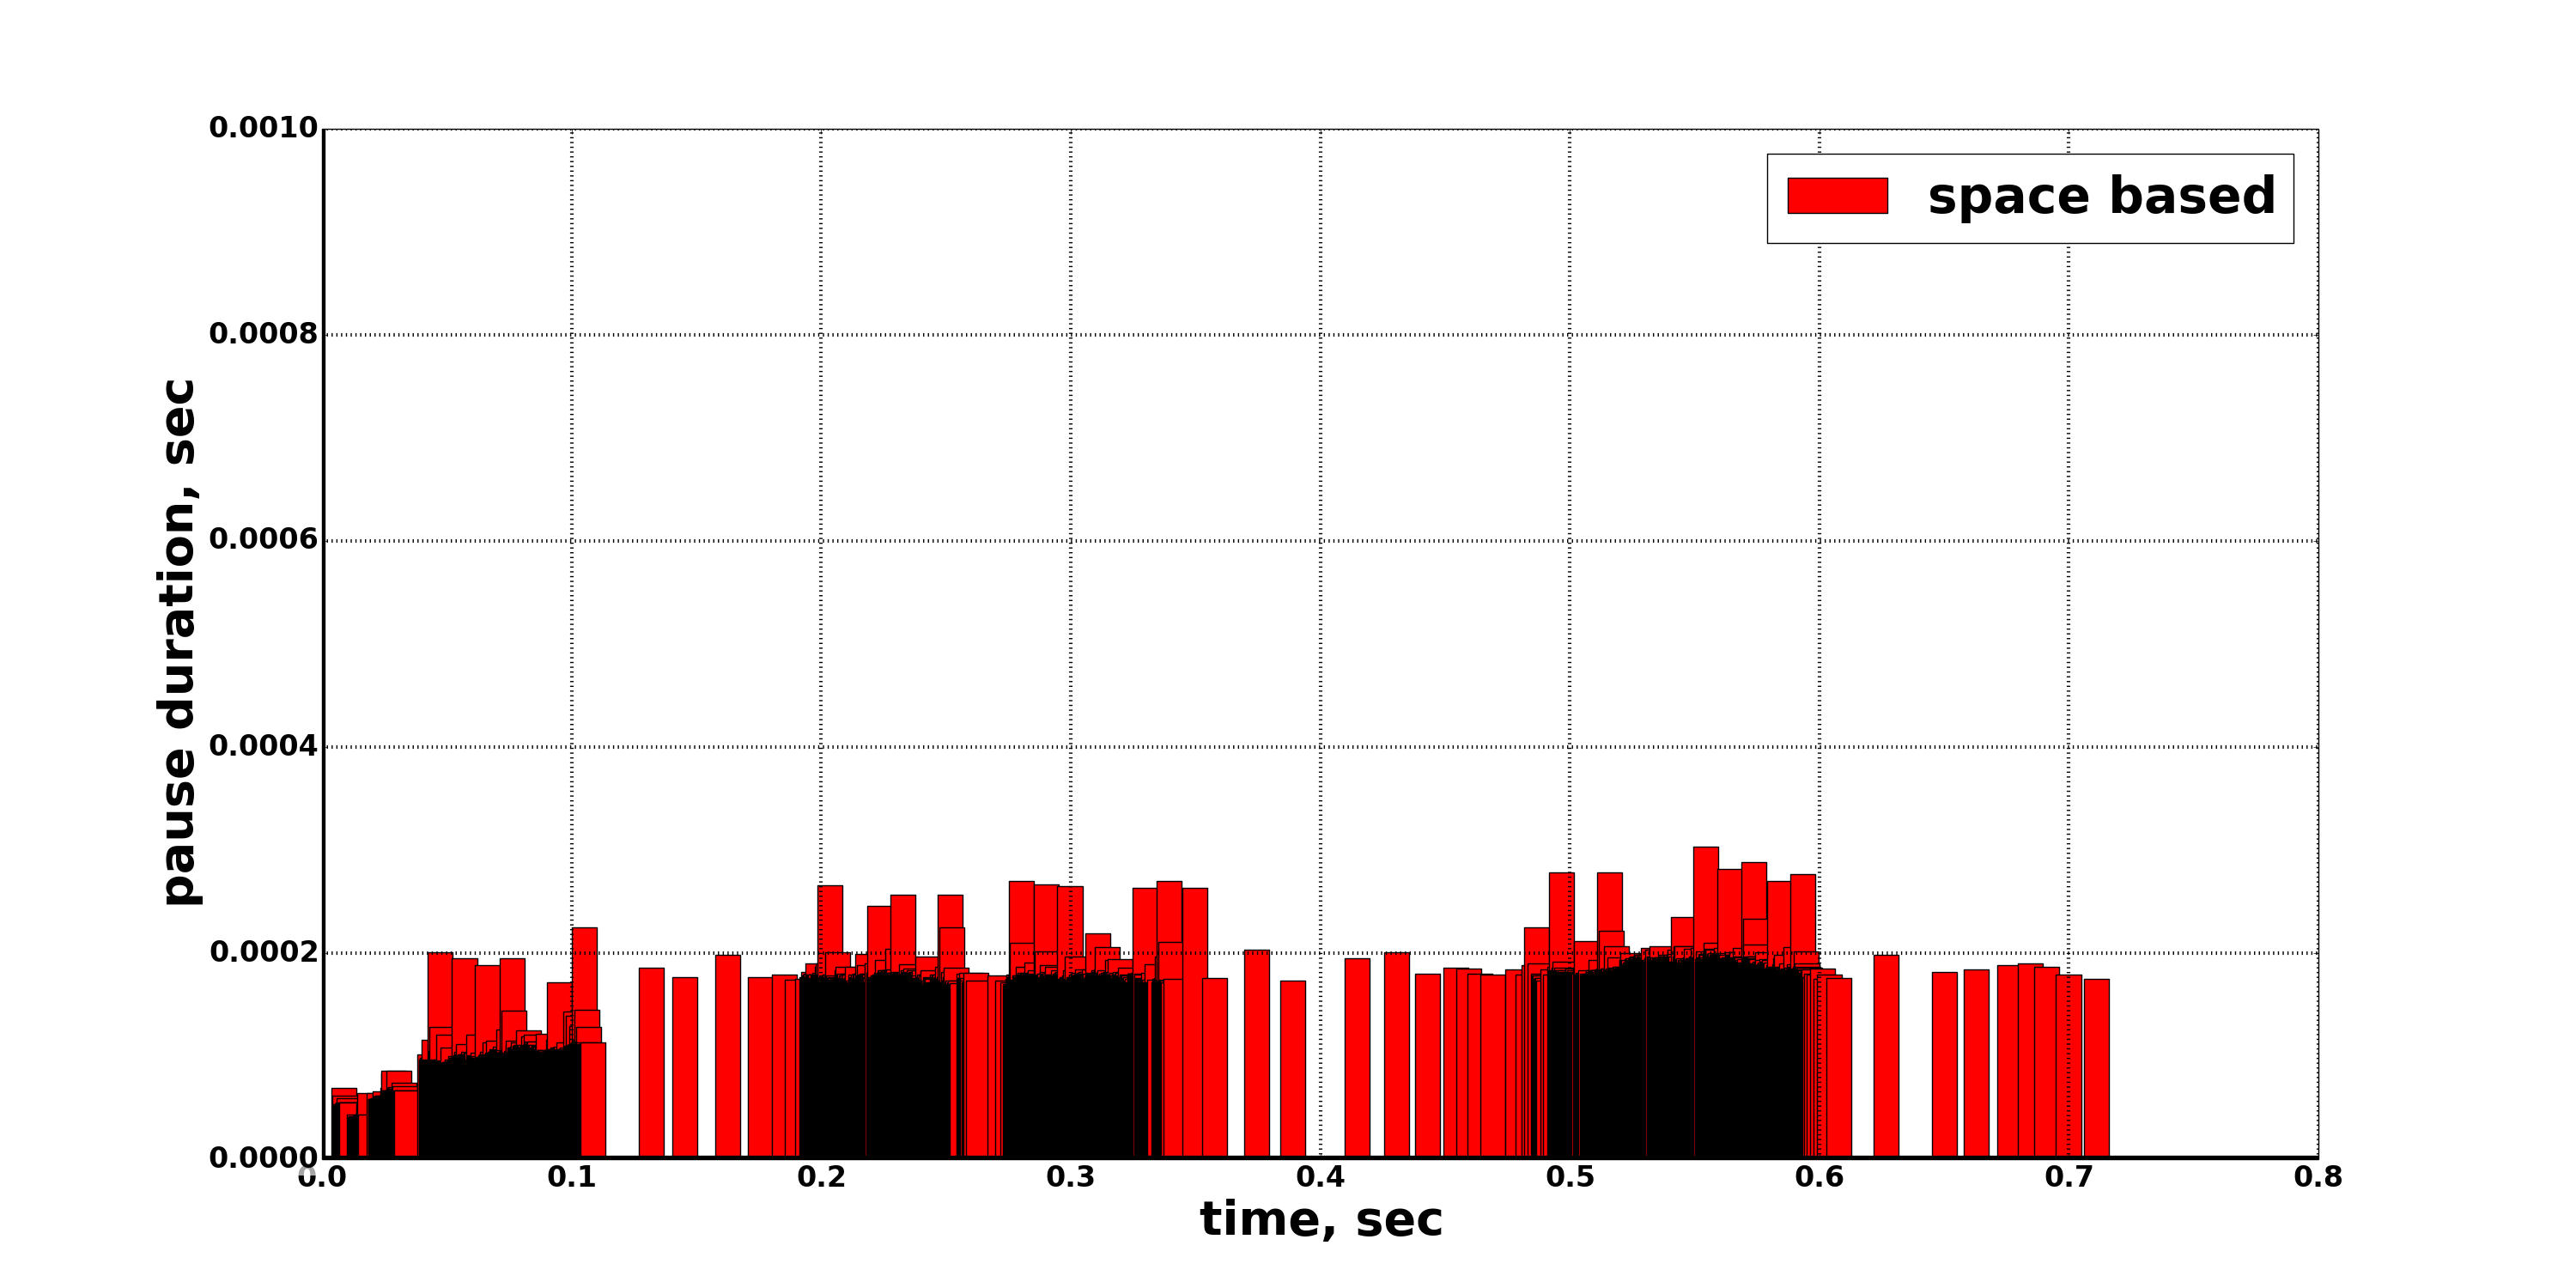
\includegraphics[width=1\linewidth]{space-based-pause-same.png}
\end{figure}

\begin{figure}[ph]
\caption{\label{pic:time-based-pause}распределение пауз при работе time based}
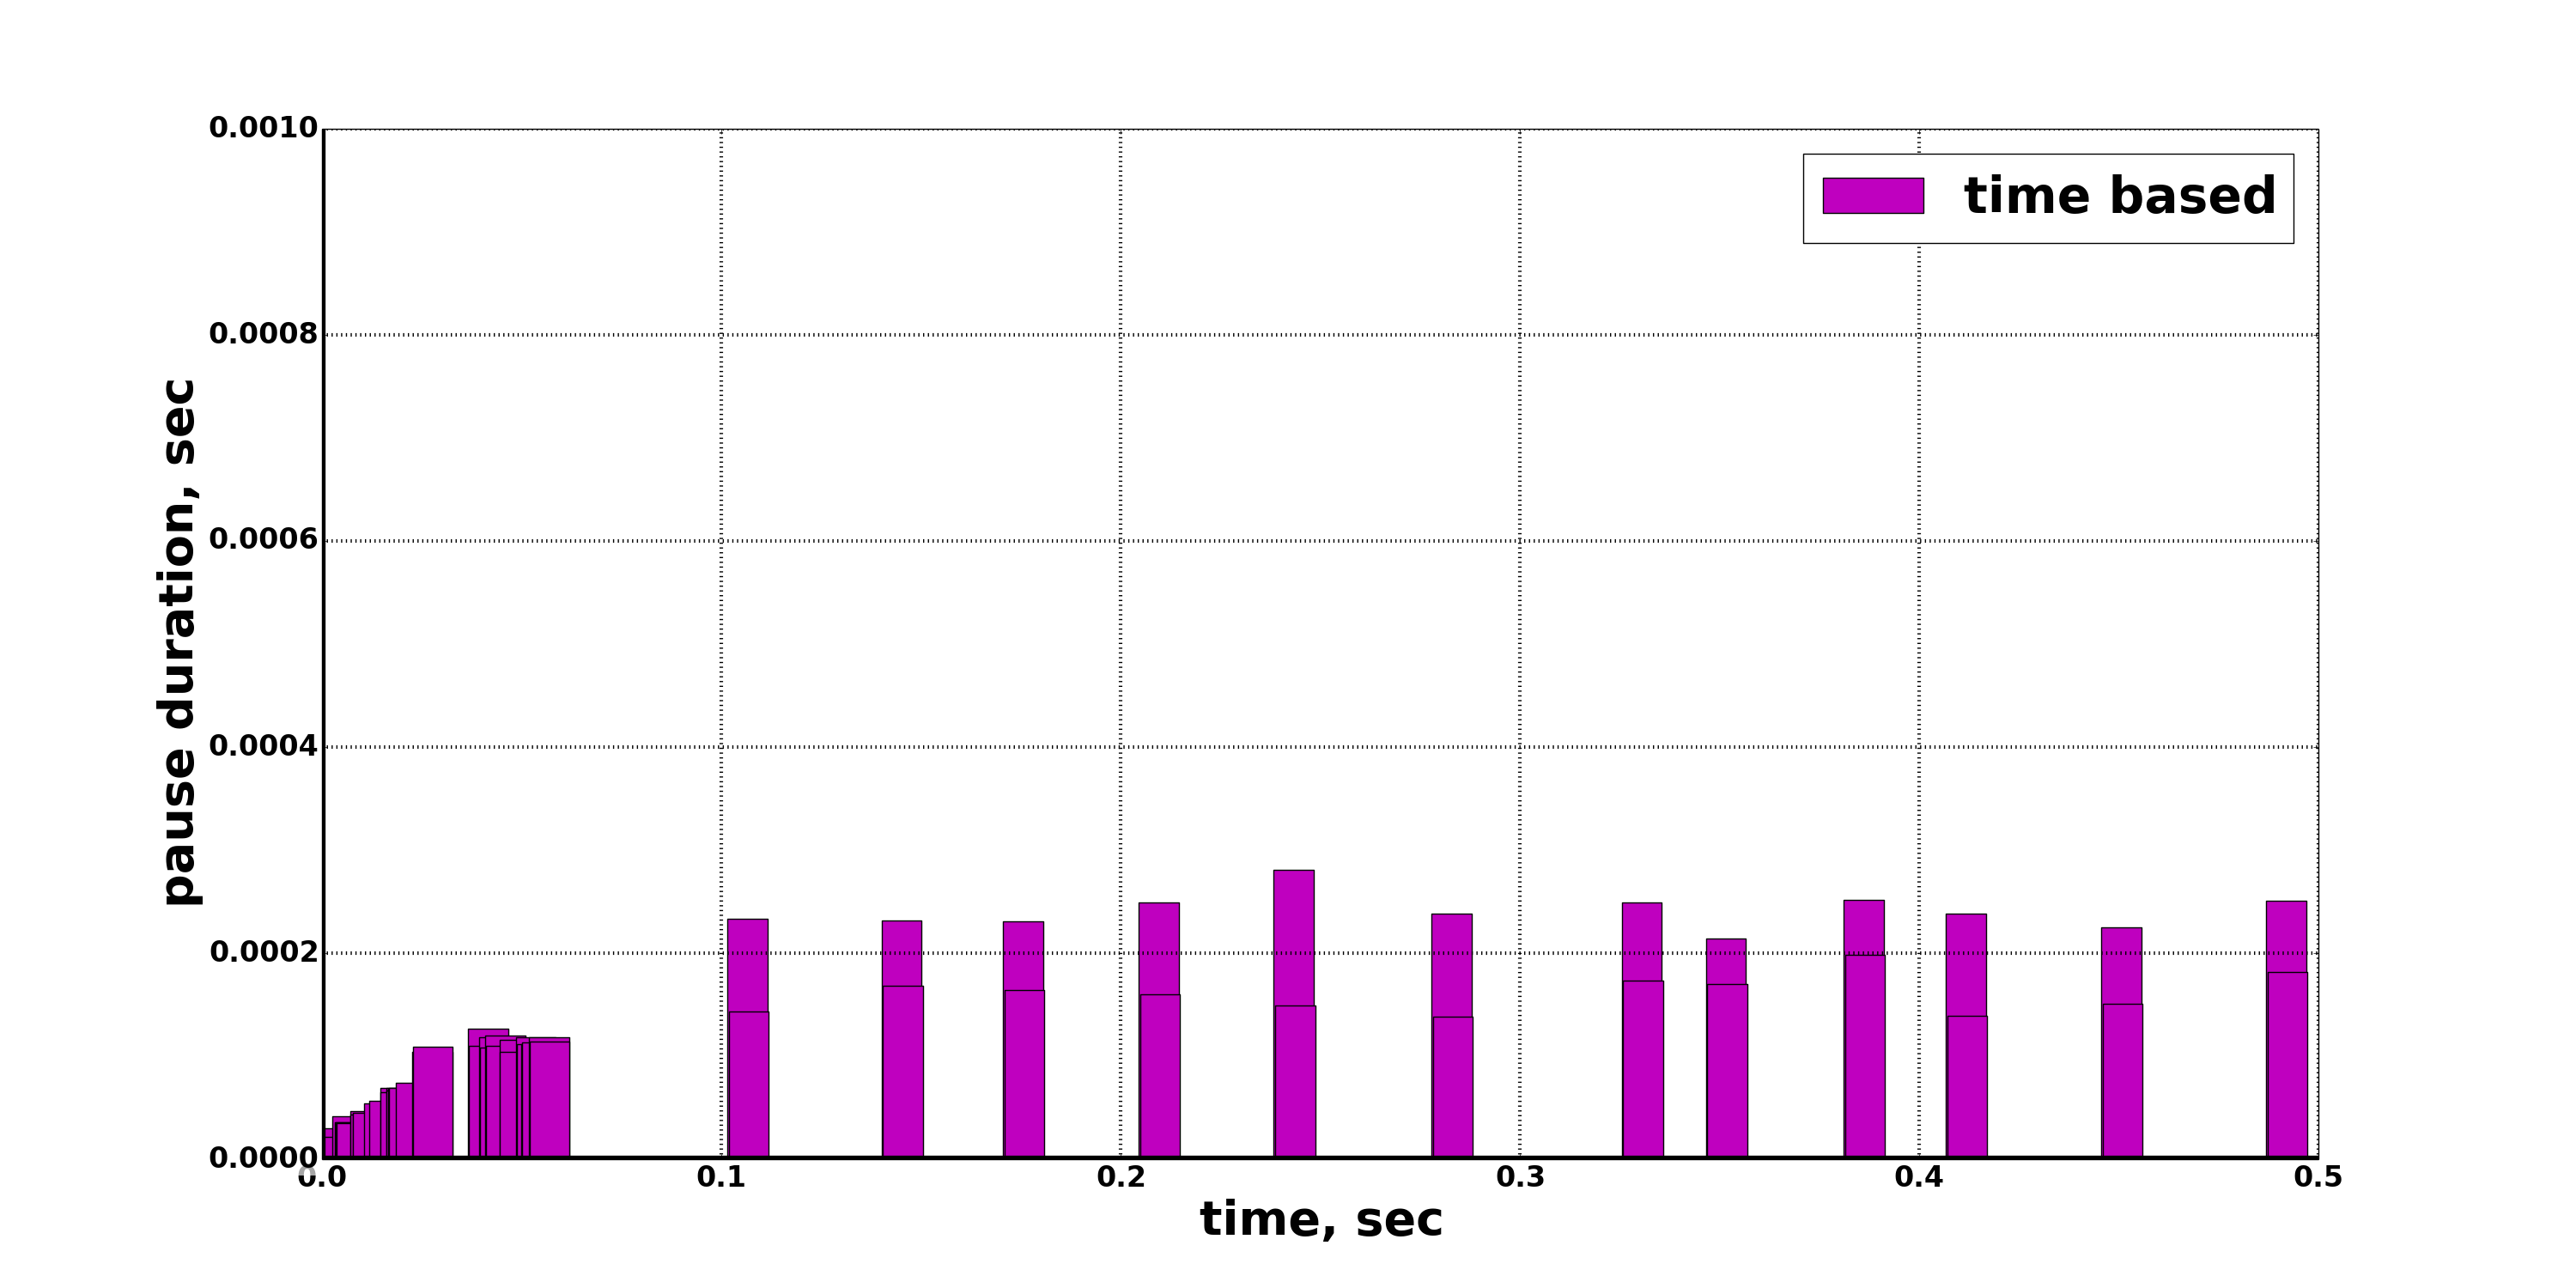
\includegraphics[width=1\linewidth]{time_based.png}
\end{figure}

\begin{figure}[ph]
\caption{\label{pic:pause-bdw}распределение пауз при работе bdw}
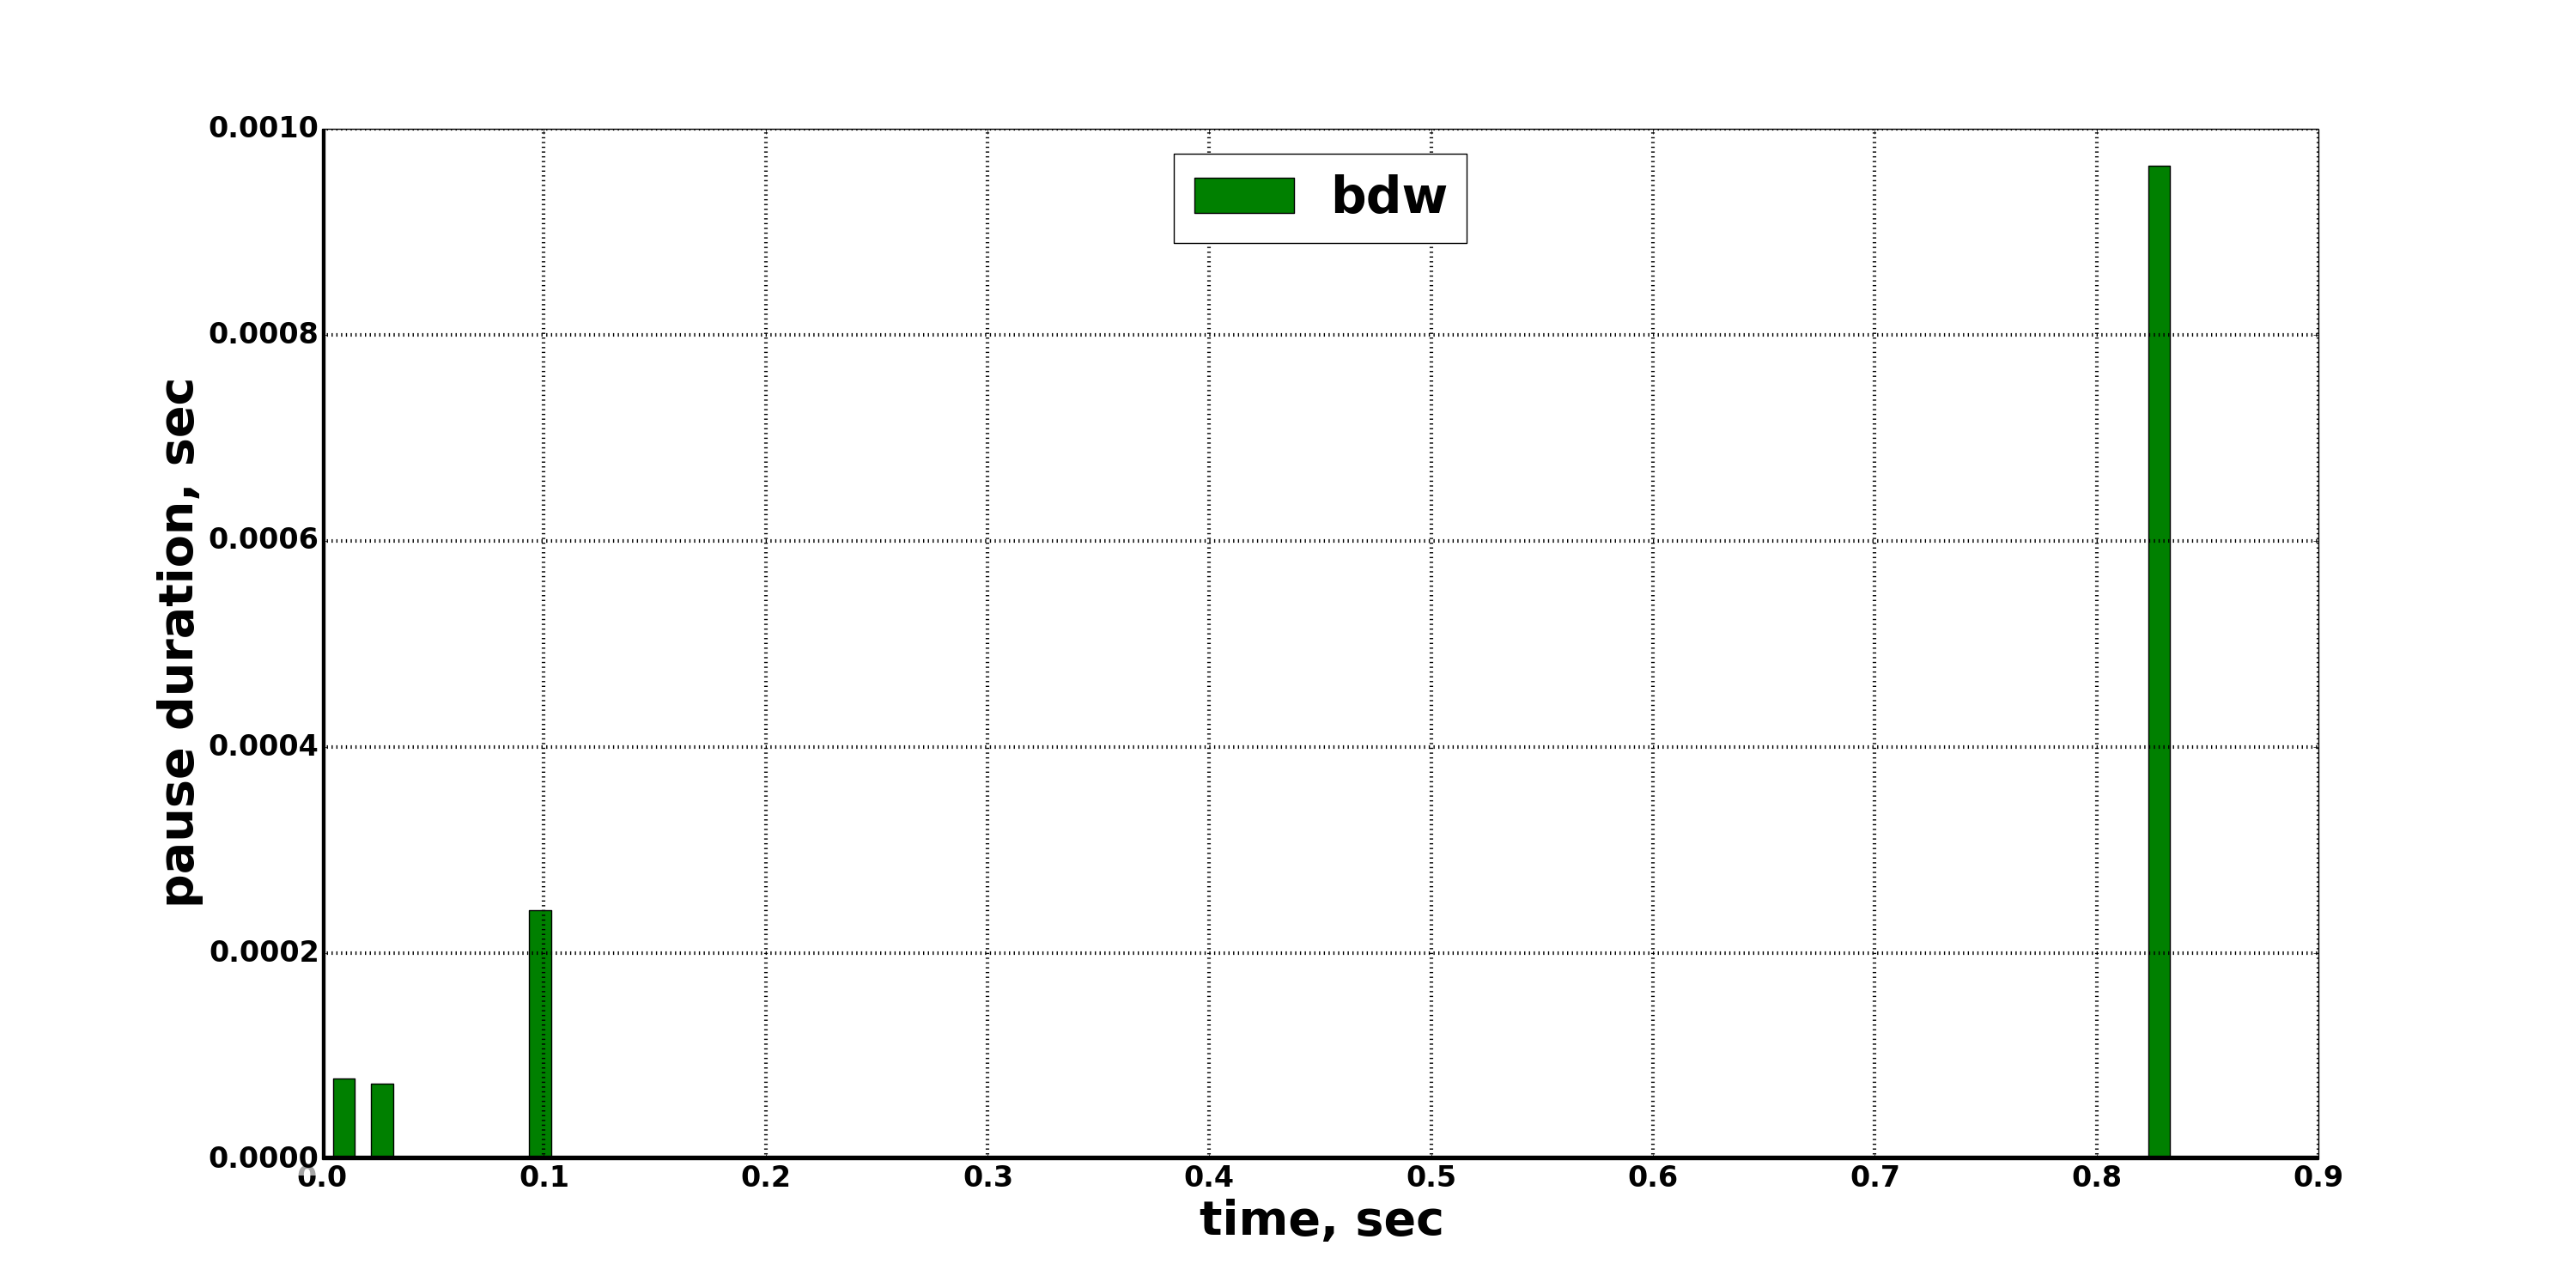
\includegraphics[width=1\linewidth]{bdw.png}
\end{figure}

\begin{figure}[ph]
\caption{\label{pic:allocated}распределение занятой памяти при работе parser}
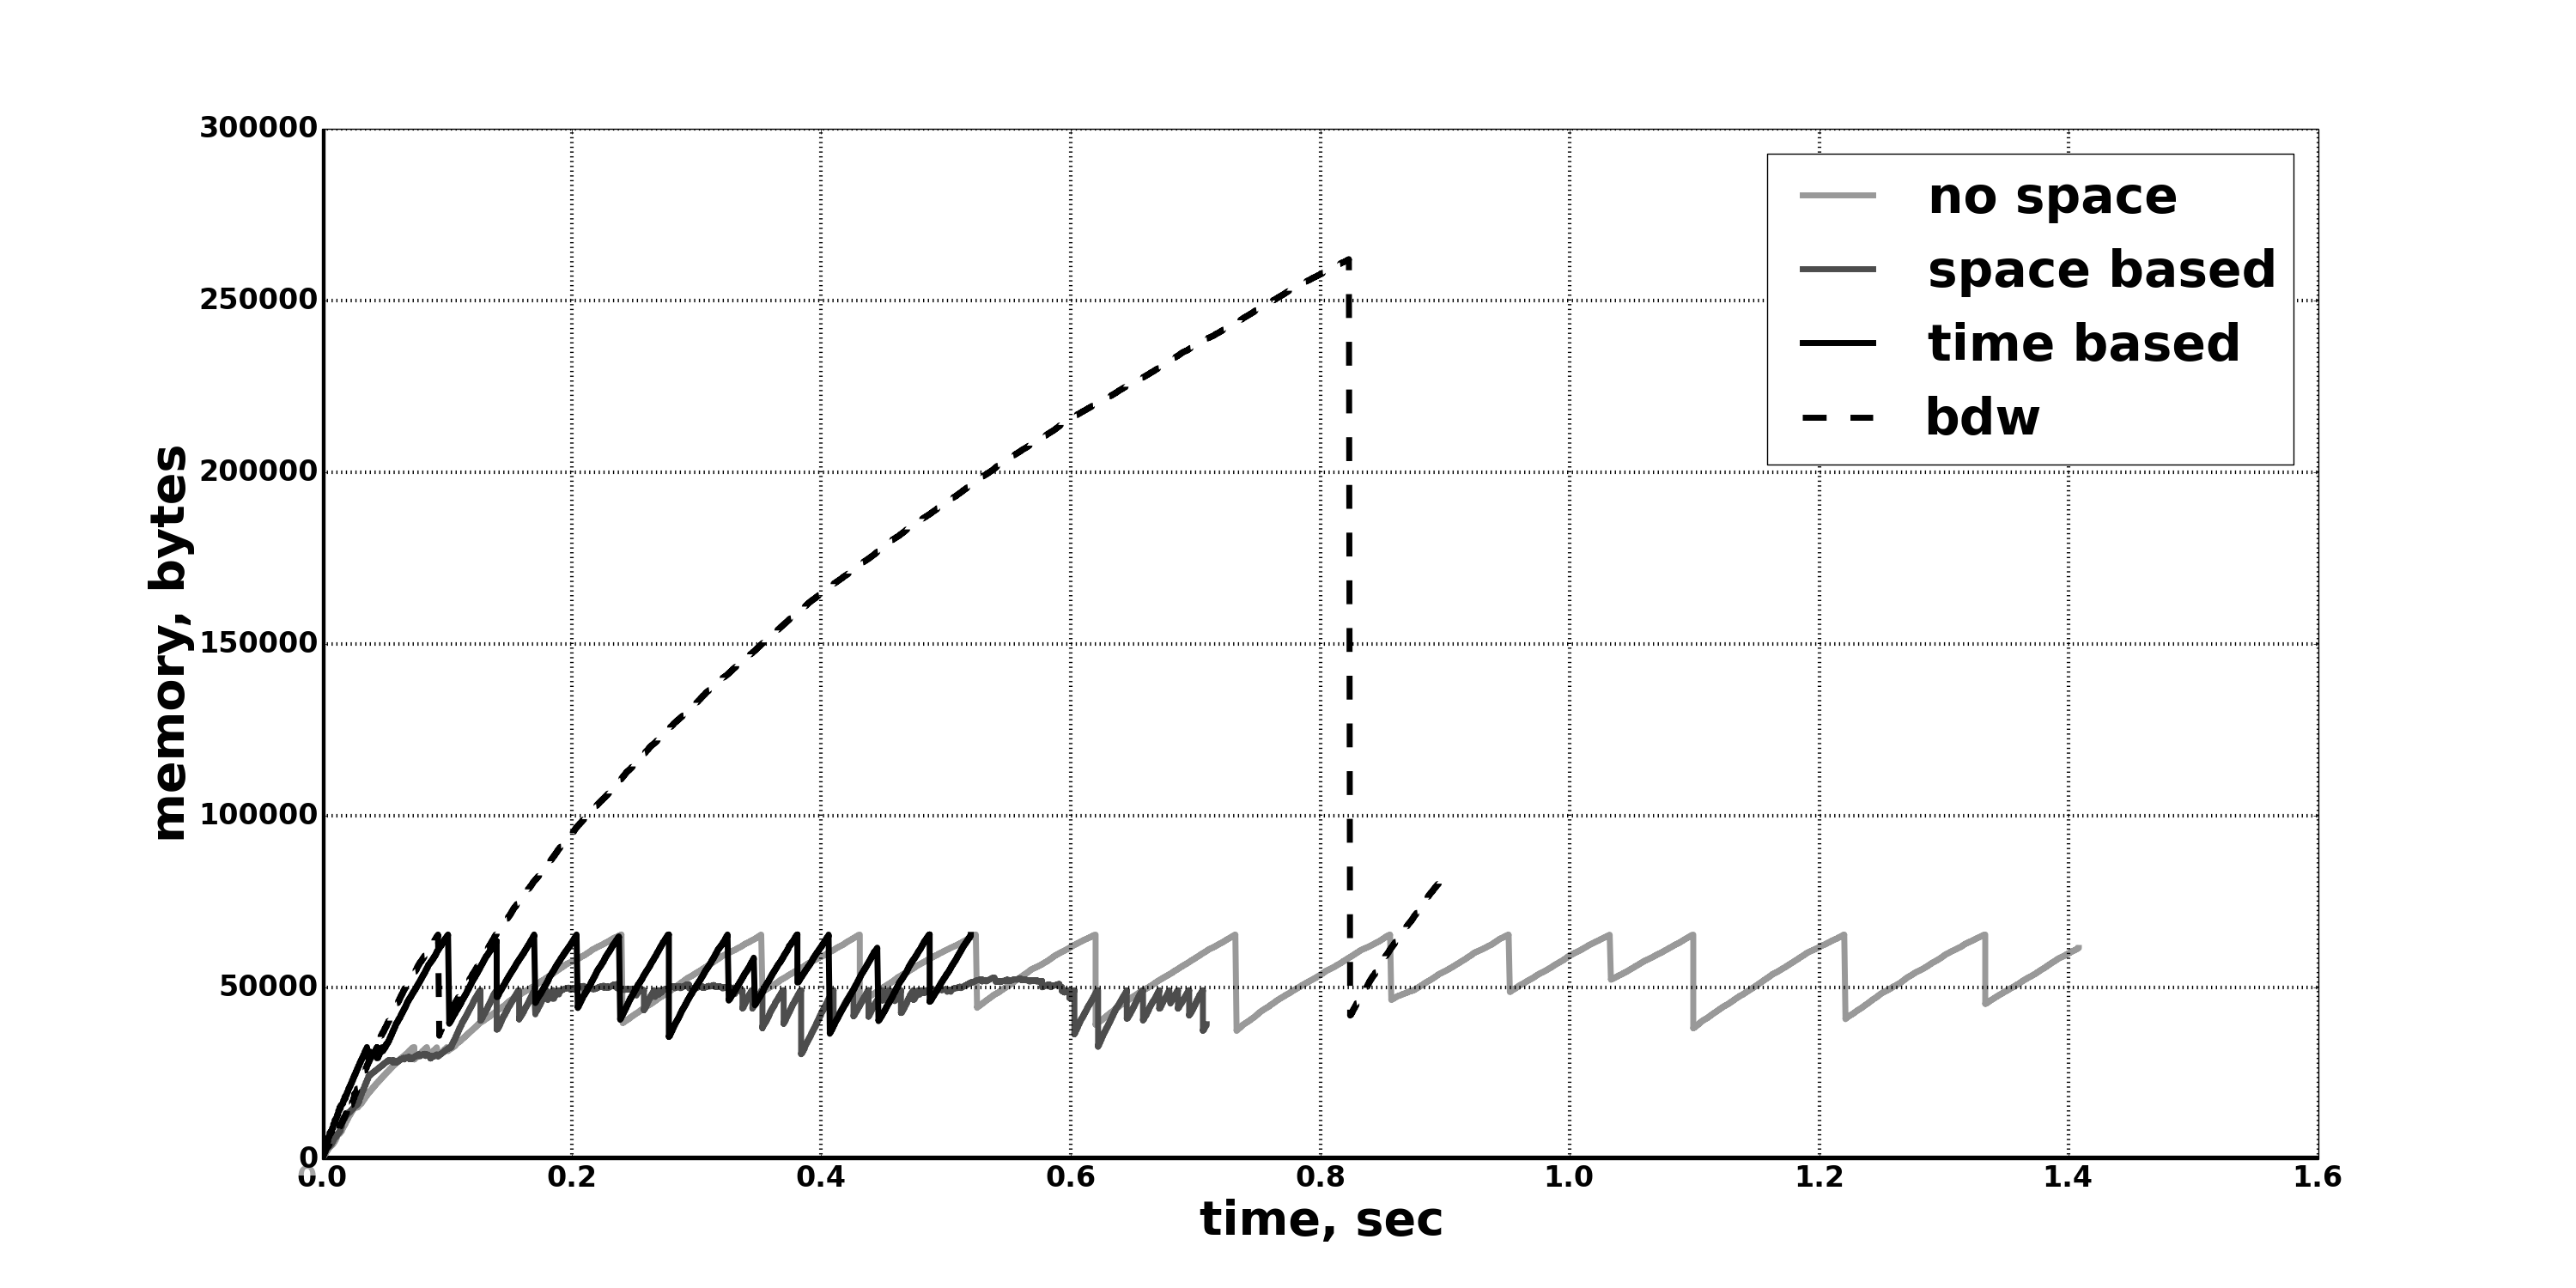
\includegraphics[width=1\linewidth]{all-allocated.png}
\end{figure}

\begin{figure}[ph]
\caption{\label{pic:perf}Время работы приложения с различными дисциплинами сборки мусора}
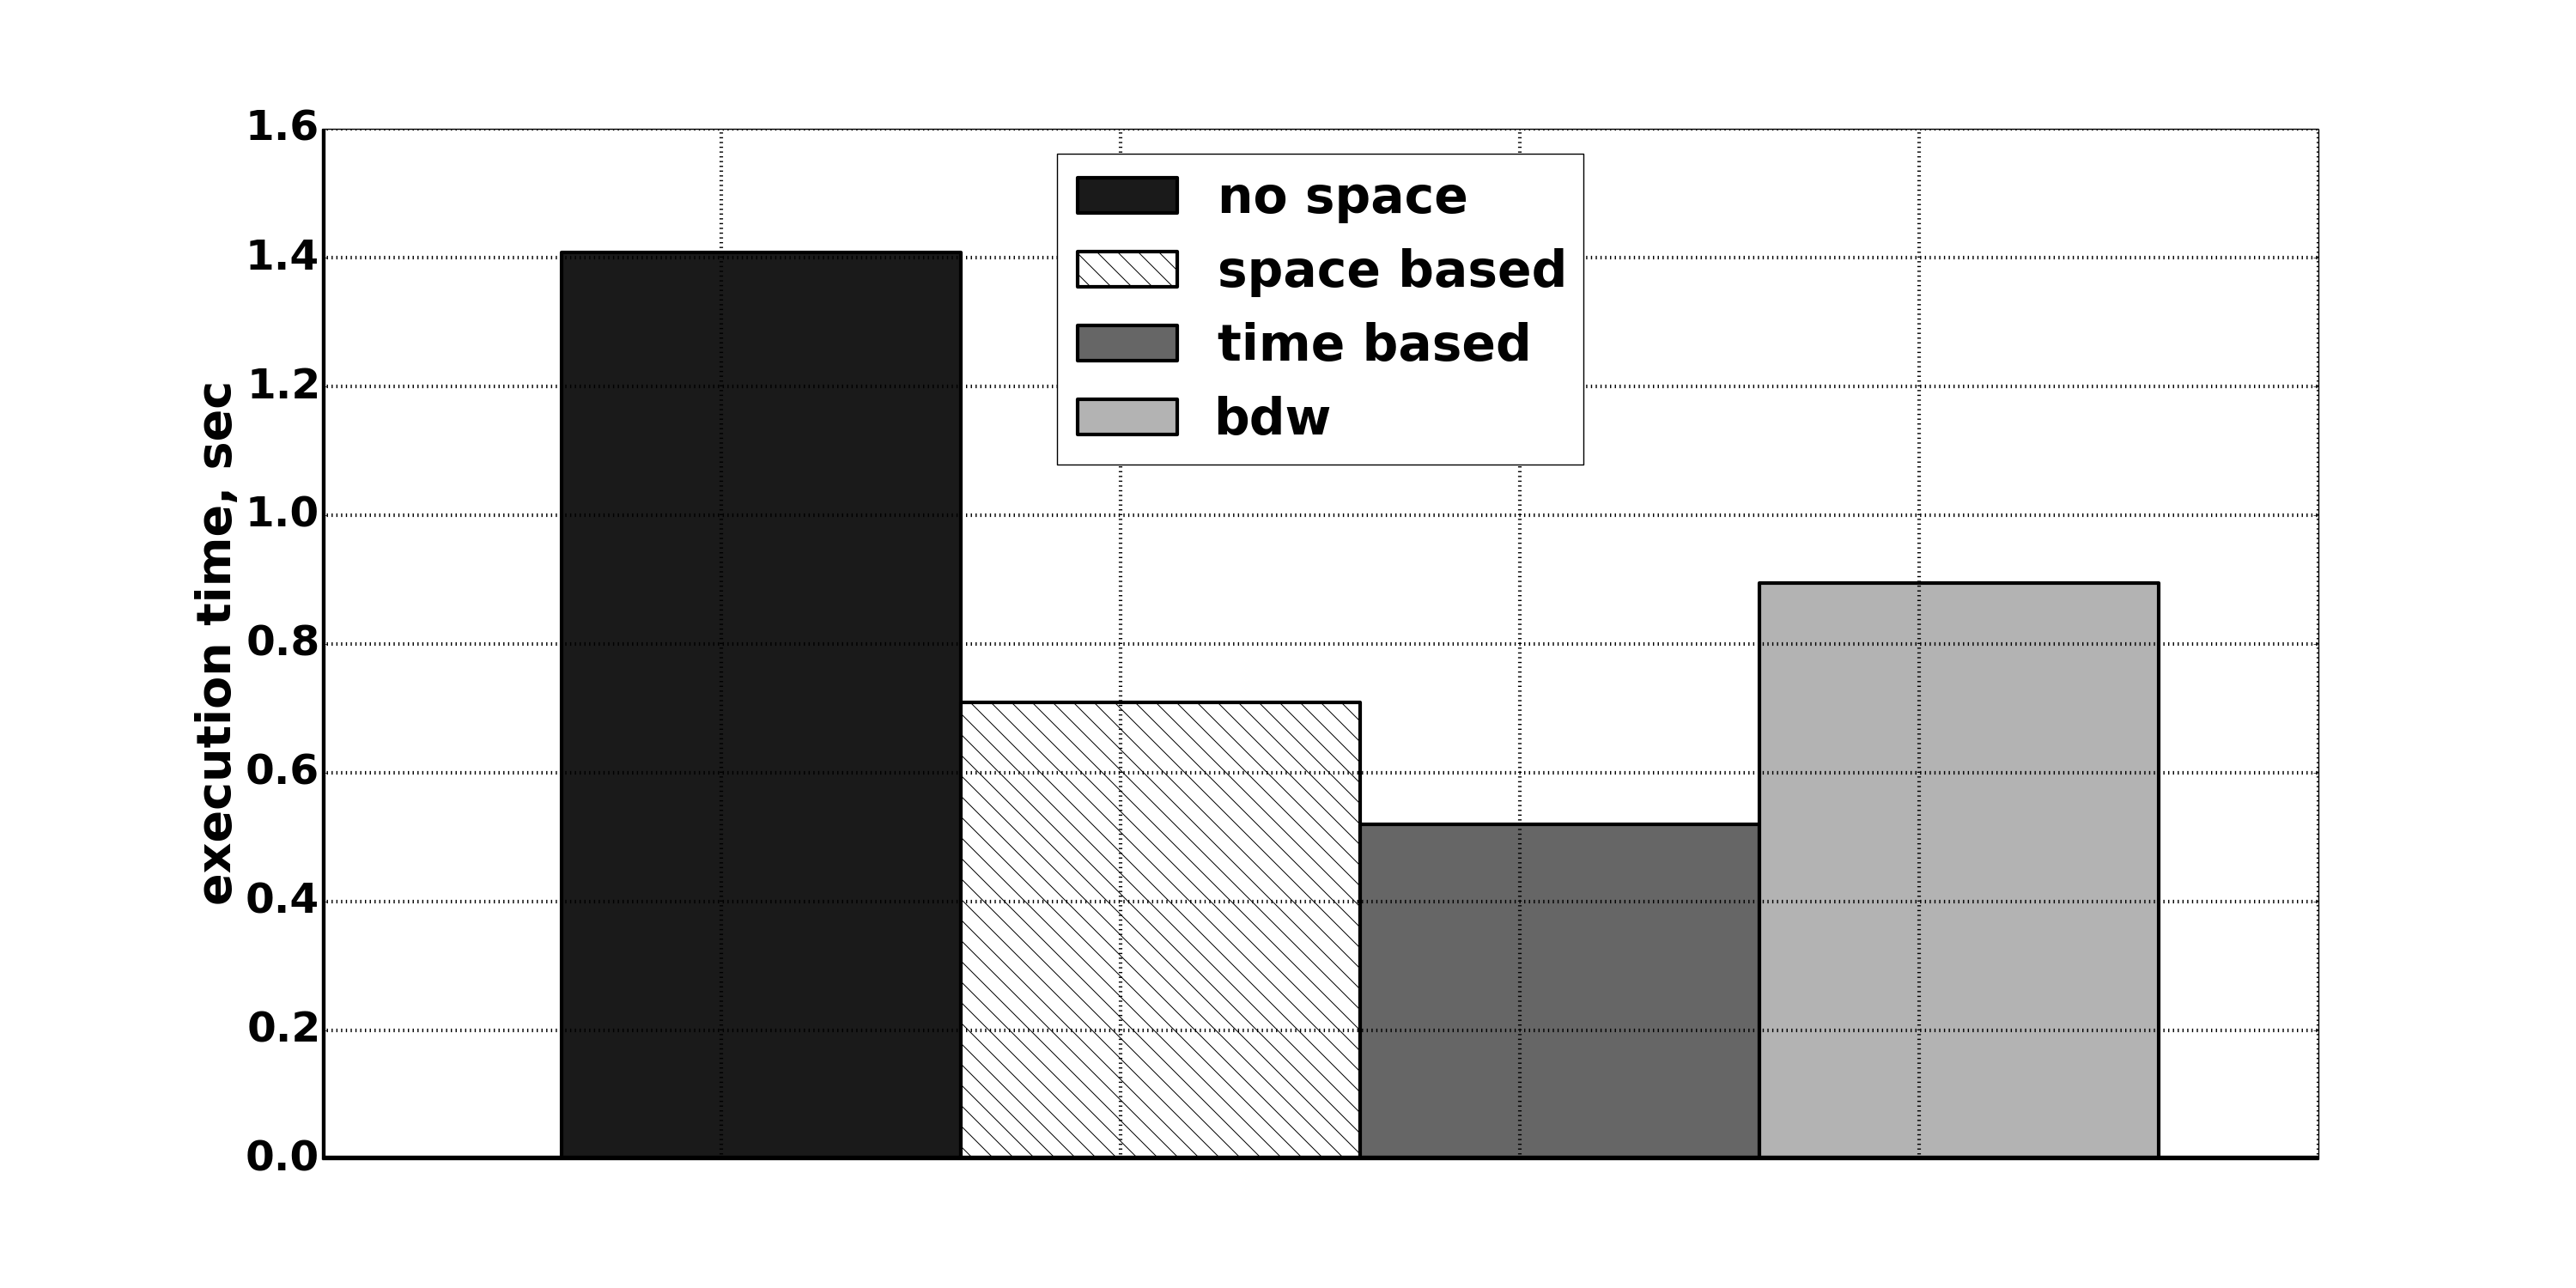
\includegraphics[width=1\linewidth]{perf.png}
\end{figure}


\section*{Заключение}
Результатом данной работы явилась реализация
четырёх критериев инициирования сборок мусора для сборщика мусора для инфраструктуры
построения компиляторов LLVM.
Реализация позволяет задавать различные параметры непосредственно при запуске
приложения: дисциплину вызова сборщика мусора и параметры, соответствующие этой
дисциплине, первоначальный размер кучи и то, во сколько раз она будет расширена при необходимости.

Различные конфигурации сборщика мусора были протестированы при работе приложения на
подмножестве языка OСaml, являющимся синтаксическим анализатором для ``игрушечного языка'',
что помогло обнаружить и исправить несколько ошибок в реализации сборщика мусора.

\pagebreak
\bibliographystyle{ugost2008ls}
\bibliography{coursework4.bib}
\end{document}
